\documentclass[12pt]{article}

\setlength{\oddsidemargin}{-0.25 in}
\setlength{\evensidemargin}{-0.25 in}
\setlength{\topmargin}{-0.9 in}
\setlength{\textwidth}{7.0 in}
\setlength{\textheight}{9.0 in}
\setlength{\headsep}{0.75 in}
\setlength{\parindent}{0.0 in}
\setlength{\parskip}{0.0 in}

\usepackage{graphicx}
\usepackage{wrapfig}
\usepackage{color}
\usepackage{caption}
\usepackage{subcaption}

\captionsetup{justification=centering}

\begin{document}
\begin{center}
Analysis of Minimum Spanning Trees in Random Graphs \\
George Zhang, Fanney Zhu \\
CS124 Programming Assignment 1 Writeup \\
https://github.com/gzhang01/cs124prog/tree/master/prog1 \\
\end{center}

\bigskip

\textbf{Abstract}

Our task was to find appropriate functions $f(n)$ to model the weight of the minimum spanning tree (MST) of a random, complete graph of $n$ edges (in the 0-dimensional case) or $n$ vertices (in the 2, 3, and 4-dimensional cases). Using C, we implemented a random graph generator and used Kruskal's algorithm to produce the MST of the graph. Our results showed that for the $d = 0$ case, we have the best fit function $f(n) = 1.2$, and for $d = 2, 3,$ and $4$, we have a best fit function of the form $f(n) = a\cdot n^{(d - 1)/d} + c$, with constants $a$ and $c$ that are dependent on the value of $d$.  \\

\bigskip

\textbf{Implementation}

Our first task was to construct the random graph generator (RGG) (see creategraph.c). We started with the 0-dimensional case, where we just assign each edge a random floating point value as a weight. To produce this random value, we seeded C's random number generator (RNG) with the current microsecond time, and used C's built-in rand() function. Of course, rand() produces a random integer between 0 and RAND\_MAX, and so we converted them to floats and normalized so our values would fall between 0 and 1. \\

We then needed some way of representing an edge. We defined a new "edge" struct that contained two integers representing the vertices of the edge and a float representing the weight. Given this, finishing the 0-dimensional RGG was simple: loop over all possible combinations of edges and create a struct with the appropriate endpoints and random weight for each one. \\

The 2, 3, and 4-dimensional cases were simple as well. We created a two dimensional (n by d) array, where each row represents a d-dimensional point. For each of the coordinates, we produced a random floating point value, and for all possible combination of two vertices, we produced an edge struct. We now had two separate functions for generating graphs, so we wrote a wrapper function that seeds the RNG and then decides with generator to call based on the input value d. To finish off the graph generators, we wrote a simple print function that would allow us to test and debug our graphs. \\

Now that we had a way to generate random graphs, we could move on to producing the MST of a given graph. We decided to go with Kruskal's algorithm, as we thought the real-world run-time of Prim's algorithm would be much longer than Kruskal's. We noticed that if we were to use Prim's algorithm, we would have to look at all vertices connected to our current MST, and we decided that repeatedly looping through all those edges would be very time-inefficient. With Kruskal's algorithm, the main time bottleneck would be sorting all the edges, but after that, we would simply take the shortest of those remaining. We decided the one-time cost of sorting was preferable to the repeated searching we would have to do with Prim's. \\\\

Our task then was to implement a disjoint set data structure (see node.c). We created a node struct containing a value, a pointer to its parent node, and a rank, and implemented the functions makeSet, find, and join. Their implementations are very similar to the pseudocode we were given in class, so we will not go into specifics here. We again created a print function to help test and debug our code. \\

With the disjoint set data structure in place, we began the implementation of Kruskal's algorithm (see mst.c). We wrote a merge sort function to sort our edges. We then took the edge with the lowest weight, determined if the two vertices are already in our MST, and if not, added the edge to our MST. To save time when running the algorithm, we kept track of how many edges we had already inserted into our MST, and stopped searching when we reached the desired number (number of vertices minus one). \\

\begin{wrapfigure}{r}{0.5\textwidth}
\vspace{-0.5cm}
\centering
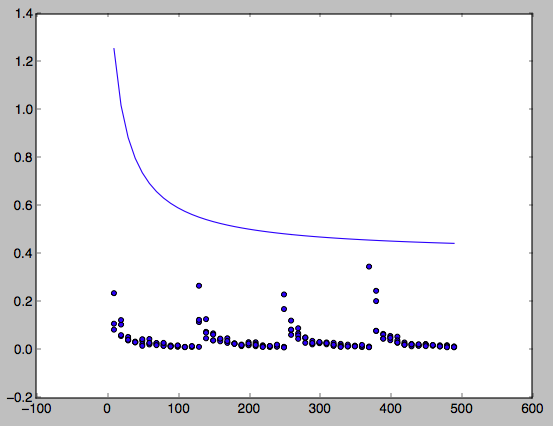
\includegraphics[width=0.4\textwidth]{img/knd0n1.png}
\caption{Actual vs. Predicted Max Edge Length in MST (n $\in$ (0, 500), d = 0)}
\end{wrapfigure}

We now had a working algorithm to find the MST of a randomly generated complete graph. Our tests for small $n$ passed easily, but unfortunately, when we tried for larger values of $n$, we ran into some memory errors. Our implementation had put certain data structures (mostly arrays) on the stack, and as $n$ increased, the amount of memory needed to store the data structures increased as well. Ultimately, we began touching memory we didn't have access to when trying to access our large arrays, triggering segmentation faults. To resolve this issue, we ended up putting all data structures on the heap and passing around pointers instead. \\

\begin{wrapfigure}{r}{0.5\textwidth}
\vspace{0cm}
\centering
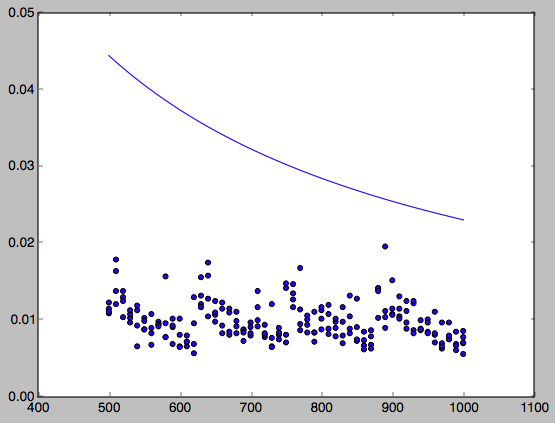
\includegraphics[width=0.4\textwidth]{img/knd0n2.png}
\caption{Actual vs. Predicted Max Edge Length in MST (n $\in$ (500, 1000), d = 0)}
\end{wrapfigure}

The next issue we faced was run time. As $n$ increased, the number of edges increased on the order of $n^2$, and so it became more and more time and memory costly to generate and sort the graph. To resolve this, we decided to prune our graph as we were generating it. We knew that once we had found a MST for a given graph, the rest of the edges that had not been searched yet had weights that were simply too high to possibly be included in the graph. We wanted to find a general estimate for this threshold, so that we could simply ignore the edge if we generate one that's too long and save time and space by not having to store and sort it. \\

\begin{wrapfigure}{r}{0.5\textwidth}
\vspace{-0.5cm}
\centering
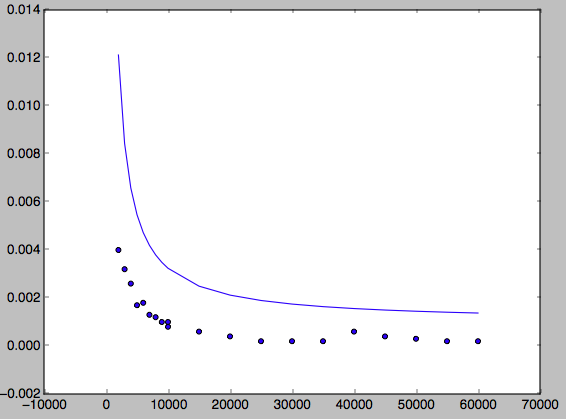
\includegraphics[width=0.4\textwidth]{img/knd0n3.png}
\caption{Actual vs. Predicted Max Edge Length in MST (n $\in$ (1000, 60000), d = 0)}
\end{wrapfigure}

Thus we wanted some function $k(n)$ that could predict, given $n$, a value $e$ such that any edge length greater than $e$ could not possibly end up in the MST. We tweaked our program to record the maximum edge length in an MST. Using some Python scripts we wrote, we plotted the maximum edge length in a MST with $n$ vertices (sample graphs on right). \\

Using these scripts, we found that this threshold not only depended on the number of vertices, $n$, but also on the number of dimensions, $d$. We decided to not find one single function that would work for any given $n, d$, but instead found 4 functions that were dependent on $d$. In addition, we found that it would have been difficult to have a good fit for the entire range we were dealing with in a single expression, and so we essentially created piecewise functions. Each of these pieces (0-500, 500-1000, 1000+) were fitted to best approximate the data. Once we implemented pruning based on these threshold functions (see threshold(n, d) in creategraph.c), we saw a mild improvement in performance for our RGGs and a significant improvement in performance for our MST generators. \\

A side note on why we believe our pruning algorithm is correct: if it were not, then the MST produced without pruning would have a smaller total weight than the MST produced with pruning. This would mean that there exists an edge in the graph that should have been included in the MST that was accidentally pruned. However, since we did not trigger our assert statement (which makes sure that the MST has $n - 1$ edges), we must have found $n - 1$ edges that satisfy the properties of the MST. Thus the edge we pruned was replaced by some other edge that must have a larger weight. But if this edge has a larger weight, then it should also have been pruned, and thus it would be impossible for us to produce an MST if we accidentally pruned an edge that should be in the correct MST. Since we do not trigger any assert statements in our running of the program, we are confident that our pruning function adequately overestimates the threshold. \\

The final major issue we came across occurred when we attempted to run our program for $n = 65536$. Our MST generator up to this point had simply allocated more than enough memory to store the complete graph (namely, enough space for nC2 edges). However, this much memory was too big for even the heap. As a result, we changed our RGGs to increase the size of the graph array as needed. In this way, we could allocate a small amount of memory to begin and add more if necessary. This also necessitated we return the number of edges we found so we could know how long the array actually was, so we could manipulate it later. \\

Ultimately, our implementation of RGGs and Kruskal's algorithm was fairly straightforward, with the exception being the optimization for large $n$. Fortunately, with our optimization, we could now run our program and have results for large $n$ in reasonable time. \\

\bigskip

\pagebreak

\textbf{Results}

We ran our program a series of times on varying values of $n$ and $d$. Since the problem statement required testing the powers of two, we ran those first. The results are shown in the table below: \\

\begin{table}[h!]
\centering
\caption{Average Weight of MST with $n$ Vertices and Dimension $d$}
\begin{tabular} {c | c | c | c | c | c  }
n&trials&d = 0&d = 2&d = 3&d = 4\\ \hline
16&10000&1.156588&2.706947&4.511162&6.137181\\
32&10000&1.184992&3.861921&7.166862&10.319945\\
64&5000&1.191658&5.433568&11.255388&17.146194\\
128&1000&1.203978&7.612868&17.600801&28.460093\\
256&300&1.203222&10.680196&27.607473&47.136620\\
512&300&1.205161&14.982530&43.397678&78.147415\\
1024&100&1.210444&21.080511&68.121613&130.106644\\
2048&30&1.204132&29.639332&107.188408&216.480087\\
4096&10&1.193288&41.676666&169.101974&360.339966\\
8192&5&1.199238&58.819538&267.806183&603.253052\\
16384&5&1.203346&83.127167&423.052734&1008.771790\\
32768&5&1.203170&117.585678&667.955505&1688.650024\\
65536&5&1.202927&166.020844&1058.974243&2829.117676\\
\end{tabular}
\label{table:1}
\end{table}

However, we decided to get a good model, we wanted a few more data points to work with. We ended up collecting the following additional data:

\begin{table}[h!]
\centering
\caption{Average Weight of MST with $n$ Vertices and Dimension $d$ (con't)}
\begin{tabular} {c | c | c | c | c | c  }
n&trials&d = 0&d = 2&d = 3&d = 4\\ \hline
1000&5&1.2058&20.6530&67.2194&127.9314\\
2000&5&1.1908&29.1936&105.1252&212.8607\\
3000&5&1.1990&35.9798&137.0924&287.7014\\
4000&5&1.2109&41.2662&166.7150&355.9292\\
5000&5&1.2077&46.0850&192.8012&418.7740\\
6000&5&1.2029&50.6606&216.8631&479.7808\\
7000&5&1.1992&54.4482&240.7518&537.3342\\
8000&5&1.1970&58.2977&263.0330&593.2632\\
9000&5&1.2033&61.7239&284.6641&647.4437\\
10000&5&1.2076&65.0109&305.5179&700.4604\\
15000&5&1.2019&79.8070&398.3995&944.5295\\
20000&5&1.2034&91.8058&481.6500&1168.7787\\
25000&5&1.2046&102.6266&558.9552&1379.5463\\
30000&5&1.2033&112.3914&630.0703&1580.5377\\
40000&5&1.2022&129.8327&762.3553&1958.2277\\
\end{tabular}
\label{table:2}
\end{table}

\pagebreak

\begin{figure}
\centering
\begin{subfigure}{.5\textwidth}
  \centering
  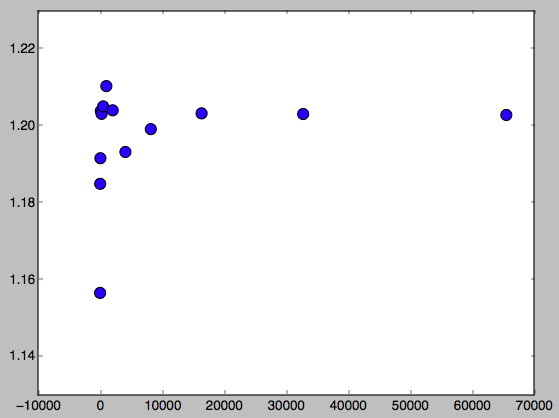
\includegraphics[width=0.8\linewidth]{img/result0.png}
  \caption{Average Weight vs. $n$ ($d = 0$)}
  \label{fig:sub1}
\end{subfigure}%
\begin{subfigure}{.5\textwidth}
  \centering
  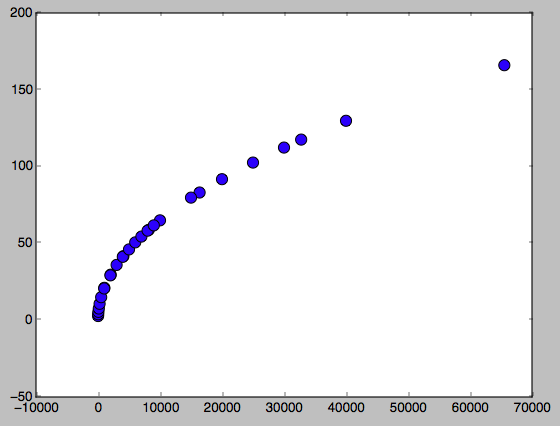
\includegraphics[width=0.8\linewidth]{img/result2.png}
  \caption{Average Weight vs. $n$ ($d = 2$)}
  \label{fig:sub2}
\end{subfigure} \\ % 
\bigskip
\begin{subfigure}{.5\textwidth}
  \centering
  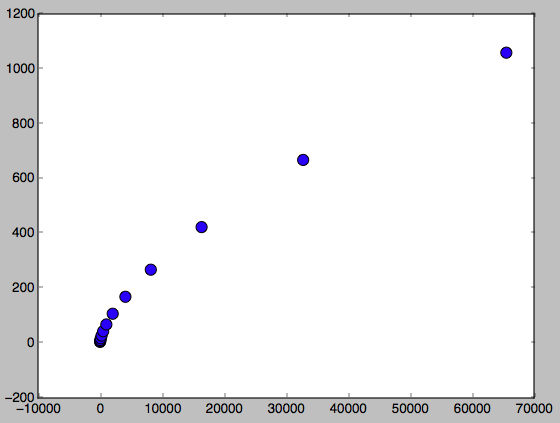
\includegraphics[width=0.8\linewidth]{img/result3.png}
  \caption{Average Weight vs. $n$ ($d = 3$)}
  \label{fig:sub3}
\end{subfigure}%
\begin{subfigure}{.5\textwidth}
  \centering
  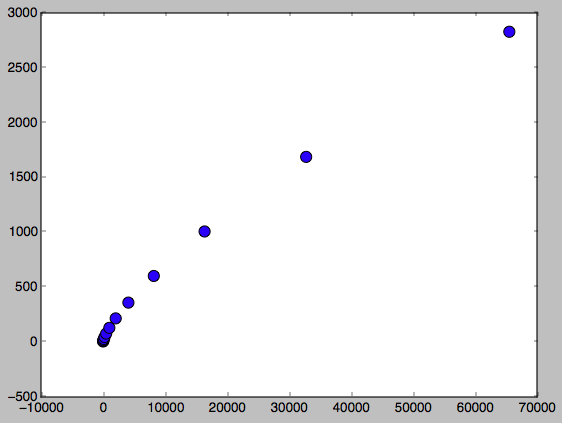
\includegraphics[width=0.8\linewidth]{img/result4.png}
  \caption{Average Weight vs. $n$ ($d = 4$)}
  \label{fig:sub4}
\end{subfigure}%
\caption{Plots of Results}
\end{figure}

We wanted to find a function $f(n)$ that could model the average weight of the MST given $n$. We notice immediately from the data that the function must depend on both $n$ and $d$. In order to find what this function should be, we graphed the data (shown above). For the $d = 0$ case, if we ignore some initial noise for small values of $n$, it appears that the average weight of the MST is around $1.2$. For the other cases, the relationship is not as clear. The curves look roughly like polynomial functions with fractional powers, so we attempted to fit the data to a function of the form $a \cdot x ^ b + c$. 

Using Python scripts we wrote, we got the following results:

\begin{table}[h!]
\centering
\caption{Coefficients of Best Fit Function}
\begin{tabular} {c | c | c | c }
d&a&b&c\\ \hline
2&0.6543&0.4991&0.2054\\
3&0.6780&0.6629&0.7354\\
4&0.7378&0.7439&1.6431\\
\end{tabular}
\label{table:3}
\end{table}

We notice that the exponent $b$ roughly takes the form $(d-1)/d$. Using this value of $b$, we recalculated our function to find better fits for $a$ and $c$. The table below summarizes the best fit functions we found for the four values of $d$:

\begin{table}[h!]
\centering
\caption{Best Fit Functions}
\renewcommand{\arraystretch}{1.3}
{\setlength{\tabcolsep}{15pt}
\begin{tabular} {c | c  }
d&$f(n)$\\ \hline
0&$f(n) = 1.2$\\
2&$f(n) = 0.6477n^{1/2} + 0.2858$\\
3&$f(n) = 0.6510n^{2/3}+1.9652$\\
4&$f(n) = 0.6907n^{3/4}+5.9482$\\
\end{tabular}}
\label{table:4}
\end{table}

We decided to graph the scatterplots along with their best fit for better visualization. Note that we scaled the y-axis of the 0-dimension graph to the range $[0, 2]$ so the visualization will not be as affected by noise. \\

\begin{figure}[h!]
\centering
\begin{subfigure}{.5\textwidth}
  \centering
  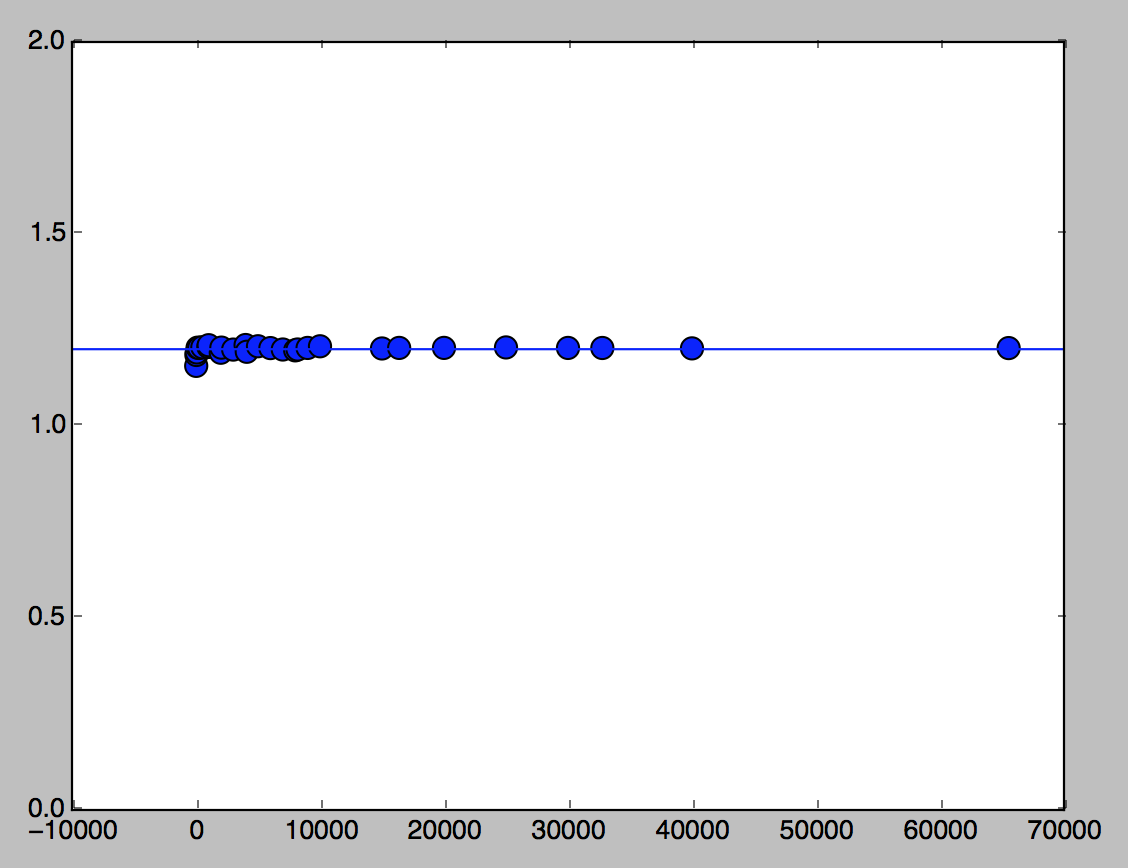
\includegraphics[width=0.8\linewidth]{img/d0_fit.png}
  \caption{Best Fit Plot ($d = 0$)}
  \label{fig:sub1}
\end{subfigure}%
\begin{subfigure}{.5\textwidth}
  \centering
  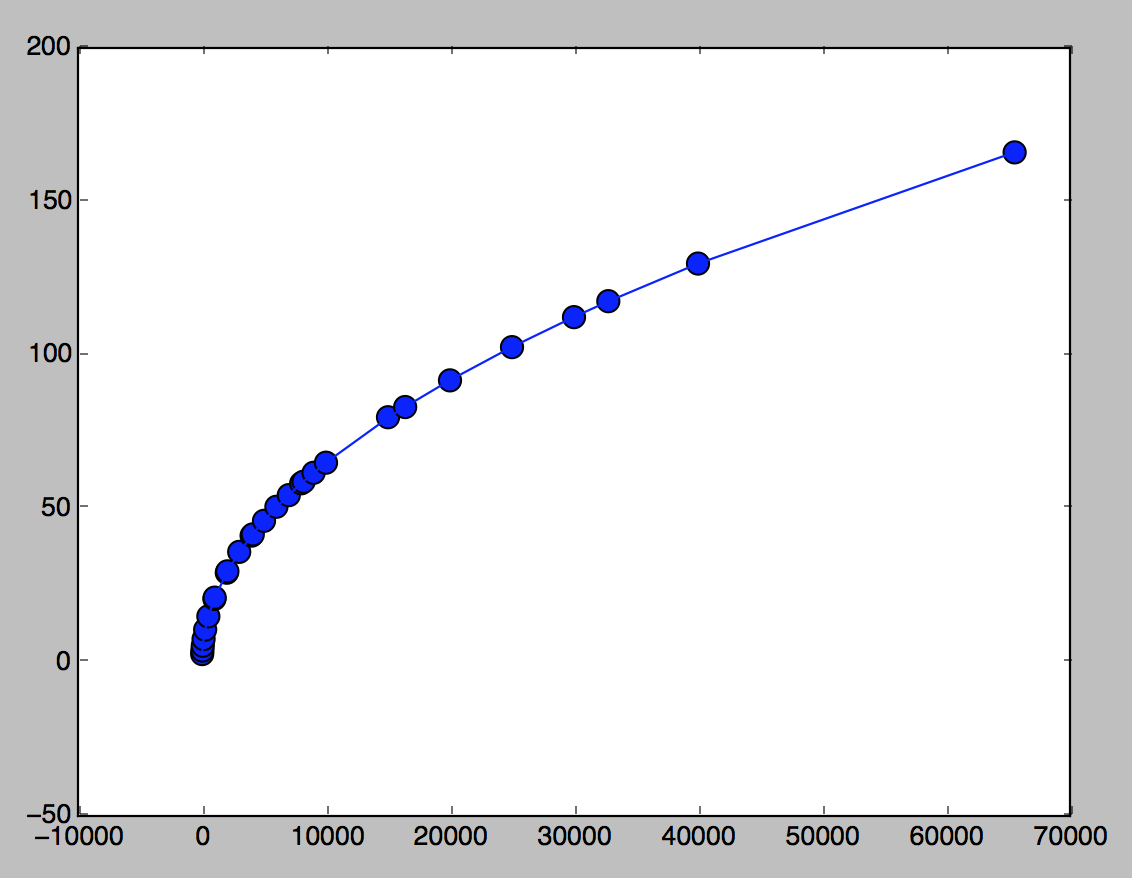
\includegraphics[width=0.8\linewidth]{img/d2_fit.png}
  \caption{Best Fit Plot ($d = 2$)}
  \label{fig:sub2}
\end{subfigure} \\ % 
\bigskip
\begin{subfigure}{.5\textwidth}
  \centering
  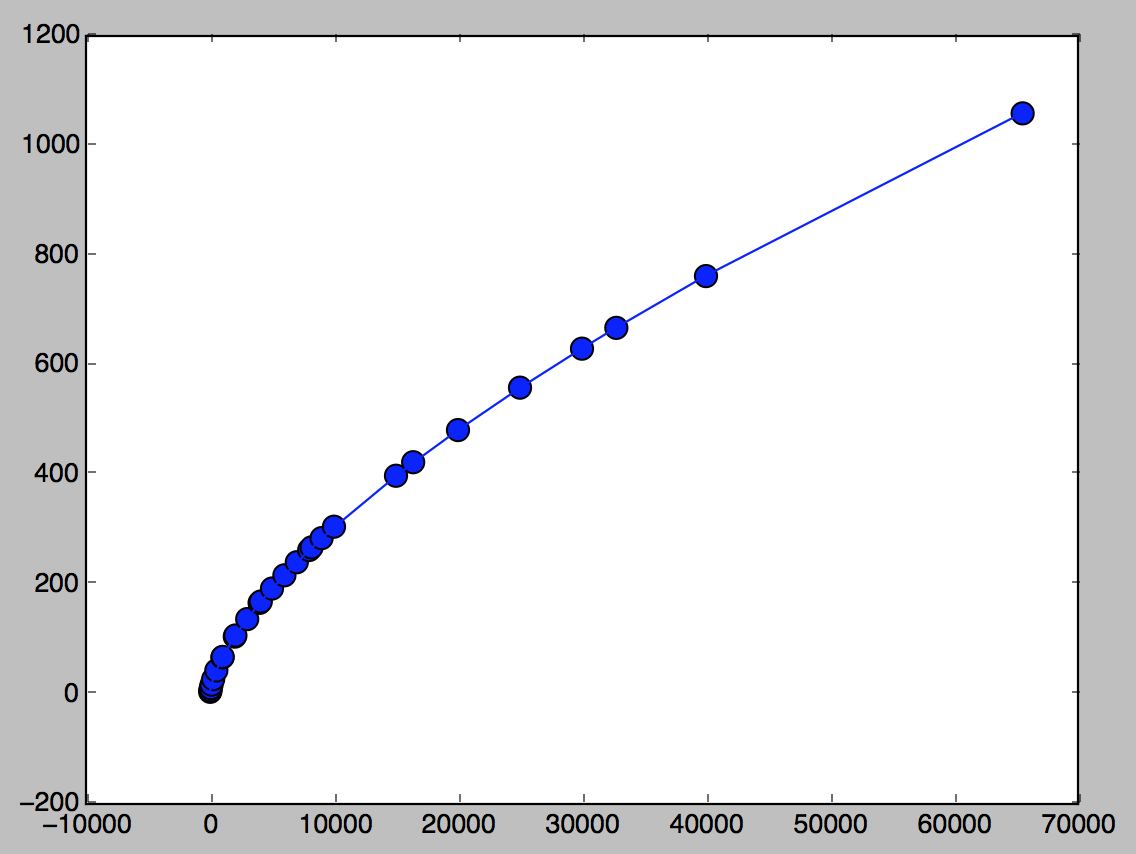
\includegraphics[width=0.8\linewidth]{img/d3_fit.png}
  \caption{Best Fit Plot ($d = 3$)}
  \label{fig:sub3}
\end{subfigure}%
\begin{subfigure}{.5\textwidth}
  \centering
  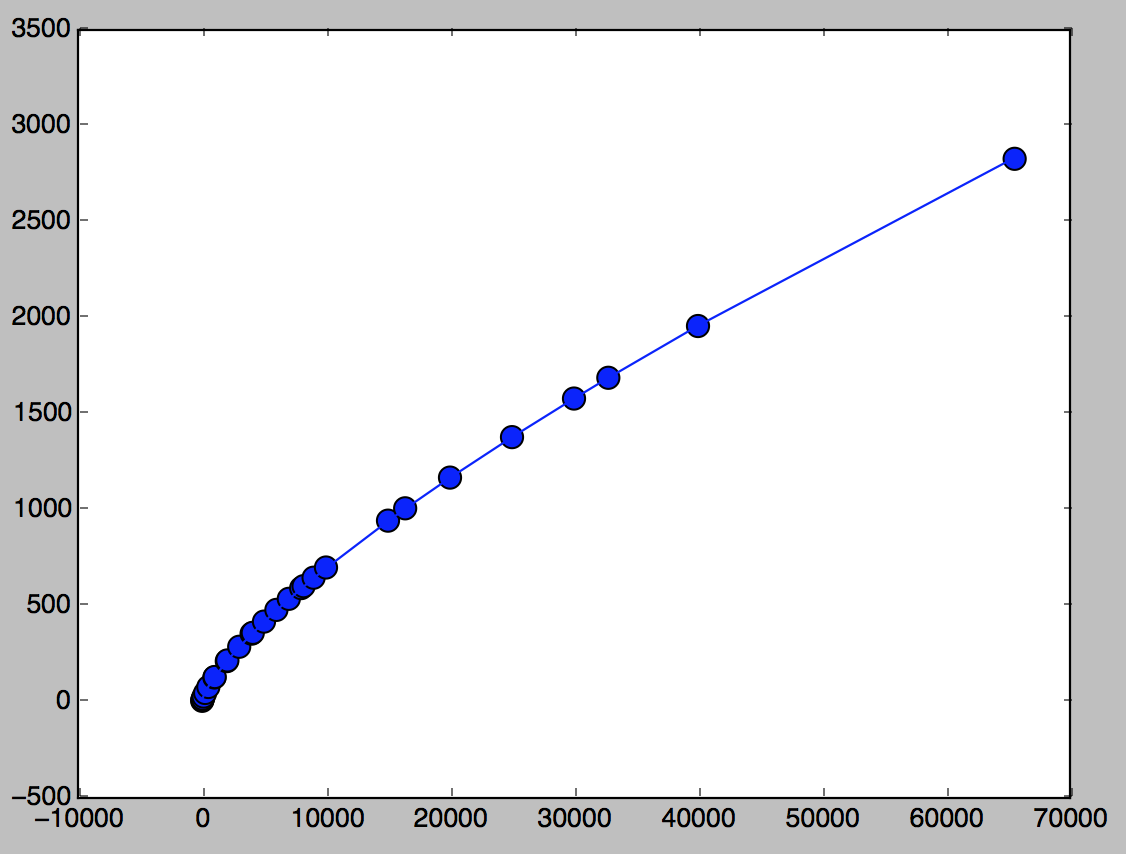
\includegraphics[width=0.8\linewidth]{img/d4_fit.png}
  \caption{Best Fit Plot ($d = 4$)}
  \label{fig:sub4}
\end{subfigure}%
\caption{Best Fit Graphs With Data}
\end{figure}

\pagebreak

\textbf{Discussion}

The purpose of the problem was twofold: to experience some of the problems involved with implementing an algorithm and exploring how minimum spanning trees behave in random graphs. We discussed much of the former in our implementation section, and so we dedicate this discussion section to talking about our findings from the latter. \\

We were relatively surprised by the results. From the data, we see that the $d = 0$ case very obviously converges at $1.2$. Our intuition for the reason behind this is that despite the fact that we're adding more edges, the average edge length in the MST should decrease proportionally. This is because we are simply choosing edge lengths randomly on the interval from 0 to 1, and so the range of the smallest $n - 1$ edges decreases as $n$ increases. Granted our MST does not necessarily contain the smallest $n - 1$ edges, but the idea that the smallest proportion of our edges decreases remains true. \\

In the $d = 2$ case, we can consider all the points lying in the unit square. The weight of the MST, which is the lengths of all the edges in the MST, can be thought of as the amount of ink needed to draw the MST. With this analogy, we can see that as we increase the number of vertices, and thus increase the number of edges in our MST, we also increase the amount of ink we use to draw the MST. This analogy might lead us to assume that the weight of the MST should be bounded (as by the area of the unit square). As we can see from the function, this is not true. Indeed, our analogy still holds, because the weight of the MST is given by the sum of the lengths of edges drawn. In the case where $n \to \infty$, we essentially shade the entire unit square, but the linear distance of all the lines (which have width 0) is infinity. We can extend this idea to the higher dimensions to see why they grow without bound as well. \\

We find the phenomenon with the exponent to be intriguing. Unfortunately, we cannot explain the exponent at this time. Please still love us $<$3. \\

During this process, we collected a bit of data on run time of the algorithm. We do not have enough data to do a rigorous analysis, but some obvious observations are that run time greatly increases as $n$ increases (we have more edges) and run time greatly increases as $d$ increases (we have $n^2$ edges compared to $n$ edges in the $d=0$ case, and we do more math to determine the edge lengths). Of course, the run time decreased dramatically after implementing our pruning function. A breakdown of the time spent revealed that most of the time was spent creating the complete graph and not the MST. Indeed, in the $d=4, n = 65536$ case, we saw that constructing the MST given the complete graph only took $4$ seconds. This suggests we did a good job with our pruning. \\

One other observation we made was in regards to the random number generator. We started out by seeding only at the beginning of creating a complete graph. However, midway through coding, we decided to seed more often (every 25 calls to rand()). Curiously, this resulted in very different results. It is hard to discuss the $d \ne 0$ cases, as their functions grow, but in the $d = 0$ case, we saw that seeding more often did not result in convergence to $1.2$. During coding (with a single seed), we were testing very often for various values of $n$ and fairly consistently got a value of $1.2$. However, when we seeded more often, we saw more variance in the data, which made us suspect that the results were not as reliable. Thus we returned to seeding once, and we were encouraged by the final function results. 




\end{document}








